\documentclass[main.tex]{subfiles}
\begin{document}
  \section{The Model}
    \subsection{Design and Development}
      \lipsum[4]
    \subsection{Mathematical Representation}
      \lipsum[5]
    \subsection{Implementation in Mathematica}
      \lipsum[6]
    \subsection{temporary section}
    
      \begin{SCfigure}
        \centering
        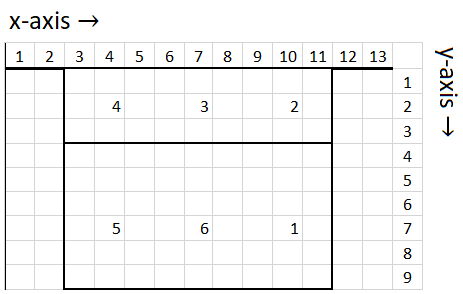
\includegraphics[width=0.5\linewidth]{figures/playingFieldGridLabelled}
        \caption{The coordinate system laid over the playing field. The net is spun at y=0 in the figure. \\
          This system is primarily used to allow the model to take player positions into account, like the distance that the setter must cover to reach the ball from their position. \\
          It is also used when noting down real world data to a format that the model can interpret.}
        \label{fig:field}
      \end{SCfigure}
      
      \begin{table}[h!]
        \label{tab:positions}
        \centering
        \caption{Basic constants defined for each position. \\
          Each position is assigned a number of constants that help calculate parameters that are in turn used to score the different positions. \\
          Note that Position 0 either refers to the setter's coordinates or to a "Dump", an attack by the setter without first setting to another player. \\
          \textbf{Ideal Contact Coordinates} describe where a player or the setter would be if they contact the ball in the ideal position. While the setter may not always be in this position, it is assumed for the model that all other players are in their ideal position when the setter makes their decision. \\
          \textbf{Ease of Attack} (also bias or \(ease_{attack}\)) is used to tune the model. It was observed for example that positions closer to the net are more likely to be set to, as they are easier to attack from successfully. \\
          \textbf{Validity} Describes when the setter is allowed to set to a position. For example, position 5 is occupied by the Libero, a player that only defends and never attacks. 
          }
        \small
        \begin{tabular}{ c | c c c }
          \hline
          Position  & Ideal Contact Coordinates & Ease of Attack & Validity \\ \hline \hline
          Setter/Dump (0) &  8,1 & 10\% & setter y=1 \\
          1 & 10,3 & 50\% & setter is front court \\
          2 & 11,1 & 90\% & setter is back court \\
          3 & 7,1 & 70\% &  always \\
          4 & 3,1 & 90\% & always \\
          5 & invalid & invalid & never\\
          6 & 7,3 & 40\% & always \\
          \hline
        \end{tabular}
        \normalsize
      \end{table}
      Most terms in the model are scaled to a fraction to ensure they do not outweigh other factors.
      \\\\
      We make use of a pressure factor which mostly describes how far ahead or behind the setter's team is in terms of points.
      
      \begin{subequations}
        \begin{equation}
          points_{Factor}=(points_{their} - points_{own})\frac{points_{higher}}{25} 
        \end{equation}
        \begin{equation}
          pressure= max( point_{Factor}, 0) + 1      
        \end{equation}
      \end{subequations}
      
      \begin{subequations}
        \begin{equation}
          distance_{max} = 8 \sqrt{2}
        \end{equation}
        \begin{equation}
          distance_{setter \to Ideal} = \sqrt{|x_{0,current} - x_{0,ideal}|^2 + 
            |y_{0,current} - y_{0,ideal}|^2}
        \end{equation}
        \begin{equation}
          ease_{Setting} = 1 - \frac{distance_{setter \to Ideal}}{distance_{max}}
        \end{equation}
      \end{subequations}
    
      \begin{subequations}
        \begin{equation}
          valid_{(p)}=\left\{  
            \begin{array}{lr} 
              1 : \text{position \emph{p} is valid} \\
              0 : \text{otherwise}
            \end{array}
          \right.
        \end{equation}
        \begin{equation}
          setScore_{(p)} = 1 - \frac{\sqrt{|x_{0,current} - x_{p,ideal}|^2 + |y_{0,current} - y_{p,ideal}|^2}}{distance_{max}}
        \end{equation}
        \begin{equation}
          score_{(p)} =  valid_{(p)} (setScore_{(p)} + pressure * ease_{Setting} * ease_{attack})
        \end{equation}
      \end{subequations}
      
\end{document}